\centering{\textbf{ข้อควรรู้เบื้องต้นเกี่ยวกับการเคลื่อนที่แบบโพรเจกไทล์}}
\tcblower
\begin{minipage}{.6\textwidth}
	\begin{itemize}[leftmargin=*]
		\item[1)] อัตราเร็วของการเคลื่อนที่ในแนวระดับ (แกน X) ($v_x$) จะมีค่าคงที่ แต่ในแนวดิ่ง (แกน Y)($v_y$) วัตถุจะมีความเร่งเนื่องจากแรงโน้มถ่วง ( g )   คงตัวอยู่ตลอดเวลา    จึงทำให้ความเร็วในดิ่งมีค่าเปลี่ยนแปลงอยู่ตลอดเวลา
	\end{itemize}
\end{minipage}
\hfill
\begin{adjustbox}{valign=c} 
	\begin{minipage}[t]{.35\linewidth}
		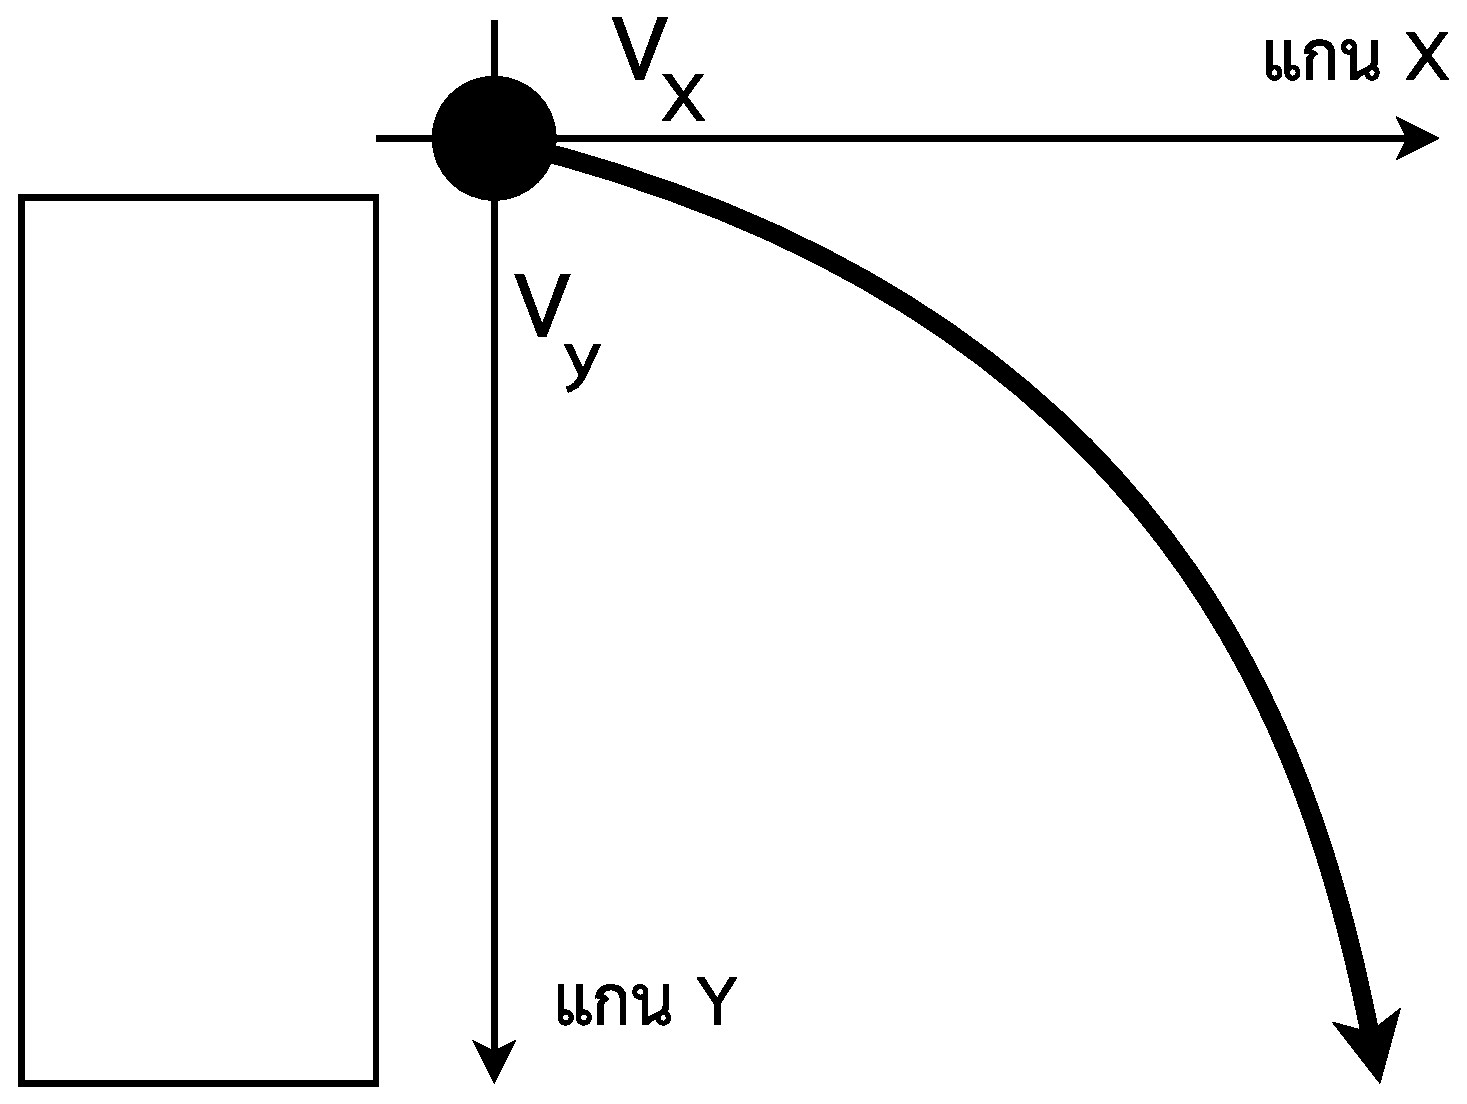
\includegraphics[width=\linewidth]{content-9-1.eps}
	\end{minipage}
\end{adjustbox}

\begin{minipage}{.6\textwidth}
	\begin{itemize}[leftmargin=*]
		\item[2)] พิจารณาการเคลื่อนที่แบบโพรเจกไทล์ชนิดโยนวัตถุจากพื้นขึ้นไปบนอากาศแล้วให้โค้งตกลงมา หากต้องการให้วัตถุเคลื่อนที่ไปในแนวระดับได้ไกลที่สุดต้องโยนวัตถุขึ้นไปในแนวเอียงทำมุม  45$^o$  กับแนวระดับ     และที่จุดสูงสุดของการเคลื่อนที่    ความเร็วของแนวดิ่ง (แกน Y) $(v_y)$ จะมีค่าเป็นศูนย์เหลือแต่ความเร็วในแนวระดับ (แกน X) $(v_x)$   เท่ากับความเร็วแนวระดับของตอนเริ่มต้น     เพราะความเร็วแนวระดับจะคงที่   ทุก ๆ จุดของการเคลื่อนที่จะมีค่าเท่ากันตลอดเวลา
	\end{itemize}
\end{minipage}
\hfill
\begin{adjustbox}{valign=c} 
	\begin{minipage}[t]{.35\linewidth}
		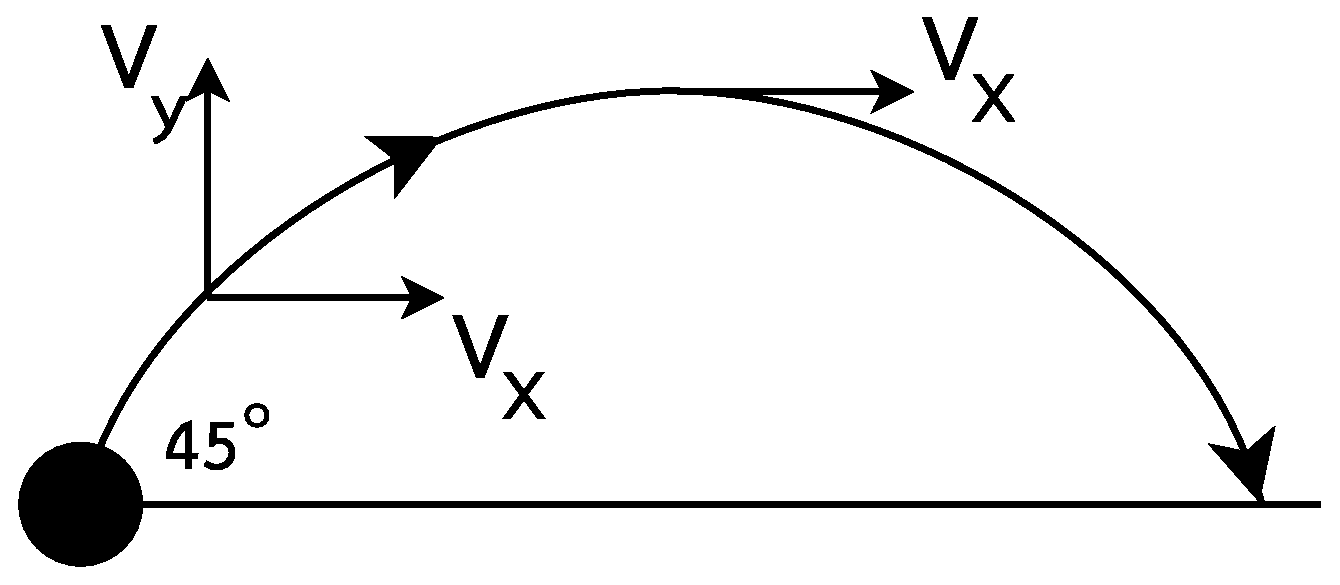
\includegraphics[width=\linewidth]{content-9-2.eps}
	\end{minipage}
\end{adjustbox}

